%% Copyright (c) 2002, 2010 Sam Williams
%% Copyright (c) 2010 Richard M. Stallman
%% Permission is granted to copy, distribute and/or modify this
%% document under the terms of the GNU Free Documentation License,
%% Version 1.3 or any later version published by the Free Software
%% Foundation; with no Invariant Sections, no Front-Cover Texts, and
%% no Back-Cover Texts. A copy of the license is included in the
%% file called ``gfdl.tex''.

\chapter{Дилемма абсолютной морали}

В половину первого ночи 27 сентября 1983 года в Usenet-группе net.unix-wizards появилось необычное сообщение за подписью \url{rms@mit-oz}. Сообщение называлось коротко и крайне заманчиво: \enquote{Новая реализация UNIX}. Но вместо некой готовой новой версии Unix читатель обнаруживал призыв:

\begin{quote}
В этот День Благодарения я начинаю писать новую, полностью совместимую с Unix операционную систему, которая будет называться GNU (GNU's Not Unix). Я буду свободно раздавать её всем желающим. Мне очень нужны ваше время, деньги, код, оборудование -- любая помощь. \endnote{Richard Stallman, \enquote{Initial GNU Announcement} (September 1983).}
\end{quote}

В глазах опытного Unix-разработчика сообщение выглядело смесью идеализма с высоким самомнением. Автор не просто брался воссоздать с нуля целую операционную систему, весьма развитую и мощную, но ещё и улучшить её. Система GNU должна была вмещать в себя все нужные компоненты вроде текстового редактора, командной оболочки, компилятора, а также \enquote{ряд других вещей}. \endnote{\textit{Ibid.}} Обещались и крайне привлекательные возможности, которых не было в существующих Unix-системах: графический интерфейс на языке программирования Lisp, устойчивая к сбоям файловая система, сетевые протоколы на основе сетевой архитектуры МТИ.

\enquote{GNU сможет запускать Unix-программы, но не будет идентичен системе Unix, -- писал автор, -- мы сделаем все нужные улучшения, которые назрели за годы работы в различных операционных системах}.

Предвидя скептическую реакцию на своё сообщение, автор дополнил его кратким автобиографическим отступлением под заголовком: \enquote{Кто я такой?}:

\begin{quote}
Я Ричард Столлман, создатель оригинального редактора EMACS, один из клонов которого вы наверняка встречали. Работаю в Лаборатории ИИ Массачусетского технологического института. Имею большой опыт разработки компиляторов, редакторов, отладчиков, командных интерпретаторов, операционных систем ITS и Lisp Machine. Реализовал независимую от терминалов поддержку экрана в ITS, а также отказоустойчивую файловую систему и две оконные системы для Lisp-машин.\endnote{\textit{Ibid.}}
\end{quote}

Так уж вышло, что затейливый проект Столлмана стартовал не в День Благодарения, как обещалось. Только в январе 1984 года Ричард с головой погрузился в разработку программного обеспечения в стиле Unix. С точки зрения системного архитектора ITS, это было всё равно что перейти от возведения мавританских дворцов к строительству пригородных торговых центров. Впрочем, разработка Unix-системы открывала и преимущества. ITS, при всей своей мощи, имела слабое место -- работала лишь на компьютере PDP-10 от компании DEC. В начале 80-х годов Лаборатория отказалась от PDP-10, и ITS, которую хакеры сравнивали с оживлённым городом, превратилась в город-призрак. Unix же был изначально разработан с прицелом на переносимость с одной компьютерной архитектуры на другую, так что подобные беды ему не грозили. Разработанный младшими научными сотрудниками AT\&T, Unix проскользнул мимо корпоративных радаров и нашёл спокойное пристанище в некоммерческом мире научных центров. Имея меньше ресурсов, чем их собратья-хакеры в МТИ, разработчики Unix приспособили свою систему к работе на зоопарке разносортного оборудования. Главным образом -- на 16-битной PDP-11, которую хакеры Лаборатории считали непригодной для серьёзных задач, но также и на 32-битных мейнфреймах вроде VAX 11/780. К 1983 году такие компании, как Sun Microsystems, создали относительно компактные настольные компьютеры -- \enquote{рабочие станции}, сравнимые по мощности со старым мейнфреймом PDP-10. На этих рабочих станциях тоже поселился вездесущий Unix.

Переносимость Unix обеспечивалась дополнительным слоем абстракции между приложениями и оборудованием. Вместо того, чтобы писать программы в машинных кодах конкретного компьютера, как это делали хакеры Лаборатории, разрабатывая программы для ITS на PDP-10, разработчики Unix использовали высокоуровневый язык программирования С, который не был привязан к конкретной аппаратной платформе. При этом разработчики сосредоточили внимание на стандартизации интерфейсов, через которые части операционной системы взаимодействовали друг с другом. В итоге получилась система, где любую часть можно было переделать, не затрагивая все остальные части и не нарушая их работу. И чтобы перенести систему с одной аппаратной архитектуры на другую, тоже достаточно было переделать только одну часть системы, а не переписывать её всю целиком. Специалисты по достоинству оценили такой фантастический уровень гибкости и удобства, поэтому Unix быстро распространился по компьютерному миру. \endnote{Marshall Kirk McKusick, \enquote{Twenty Years of Berkeley Unix,} \textit{Open Sources} (O'Reilly \& Associates, Inc., 1999): 38.}

Столлман решил создать систему GNU из-за кончины ITS, любимого детища хакеров Лаборатории ИИ. Смерть ITS была ударом для них, в том числе и для Ричарда. Если история с лазерным принтером Xerox открыла ему глаза на несправедливость собственнических лицензий, то кончина ITS подтолкнула его от неприятия закрытого софта к активному противодействию ему.

Причины гибели ITS, как и её код, уходили далеко в прошлое. К 1980 году большинство хакеров Лаборатории уже работали над Lisp-машиной и операционной системой для неё.

Lisp -- элегантный язык программирования, прекрасно подходящий для работы с данными, структура которых заранее неизвестна. Его создал пионер исследований искусственного интеллекта и создатель самого термина \enquote{искусственный интеллект} Джон Маккарти, который работал в МТИ во второй половине 50-х годов. Название языка -- сокращение от \enquote{LISt Processing} или \enquote{обработка списков}. После того, как Маккарти ушёл из МТИ в Стэнфорд, хакеры Лаборатории несколько изменили Lisp, создав его местечковый диалект MACLISP, где первые 3 буквы обозначали проект MAC, благодаря которому, собственно, и появилась Лаборатория ИИ в МТИ. Под руководством системного архитектора Ричарда Гринблатта хакеры Лаборатории разработали Lisp-машину -- специальный компьютер для выполнения программ на языке Lisp, а также операционную систему для этого компьютера -- тоже, конечно, написанную на Lisp.

К началу 80-х годов конкурирующие группы хакеров основали две компании по производству и продаже Lisp-машин. Компания Гринблатта называлась Lisp Machines Incorporated или просто LMI. Он рассчитывал обойтись без внешних инвестиций и создать чисто \enquote{хакерскую компанию}. Но большинство хакеров присоединились к Symbolics, обычному коммерческому стартапу. В 1982 году они уже полностью покинули МТИ.

Тех, кто остался, можно было по пальцам одной руки пересчитать, так что программы и машины чинились всё дольше и дольше, или не чинились вовсе. И что хуже всего, по словам Столлмана -- в Лаборатории начались \enquote{демографические изменения}. Хакеры, которые и раньше были в меньшинстве, почти исчезли, оставив Лабораторию в полное распоряжение преподавателей и студентов, чьё отношение к PDP-10 было откровенно неприязненным.

В 1982 году Лаборатория ИИ получила замену своему 12-летнему PDP-10 -- DECSYSTEM 20. Приложения, написанные для PDP-10, работали на новом компьютере без проблем, потому что DECSYSTEM 20 был, по сути, обновлённым PDP-10, но вот прежняя операционная система совсем не подходила -- ITS нужно было портировать на новый компьютер, а значит -- почти полностью переписать. И это в то время, когда из Лаборатории ушли почти все хакеры, которые могли бы этим заняться. Так что на новом компьютере быстро воцарилась коммерческая операционная система Twenex. Те немногие хакеры, что остались в МТИ, могли только смириться с этим.

\begin{figure}[ht] \centering
  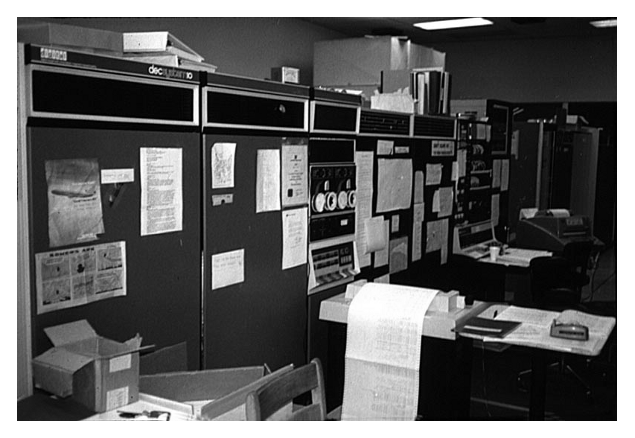
\includegraphics{KL10_1979}
  \caption{Компьютер PDP-10 с процессором KL-10, Стэнфордская лаборатория ИИ, 1979 год. Такая же машина была в Лаборатории МТИ.}
\end{figure}

\enquote{Без хакеров, которые потянули бы создание и сопровождение операционной системы, мы обречены, -- говорили сотрудники факультета и студенты, -- нам нужна коммерческая система, которую поддерживает какая-нибудь компания, чтобы она сама решала проблемы с этой системой}. Столлман вспоминает, что этот аргумент оказался жестокой ошибкой, но в тот момент он звучал убедительно.

Поначалу хакеры видели в Twenex очередное воплощение авторитарной корпократии, которое так и хотелось сломать. Даже в названии отразилась неприязнь хакеров -- вообще-то, система называлась TOPS-20, указывая на преемственность с TOPS-10, тоже коммерческой системой DEC для PDP-10. Но архитектурно TOPS-20 не имела ничего общего с TOPS-10. Её сделали на основе системы Tenex, которую компания Bolt, Beranek and Newman разработала для PDP-10. \endnote{Источники: интервью Ричарда Столлмана и электронные письма Джеральда Сассмена}. Называть систему \enquote{Twenex} начал Столлман, просто чтобы не называть её TOPS-20. \enquote{Системе было далеко до топовых решений, так что называть её официальным именем язык не поворачивался, -- вспоминает Столлман, -- поэтому я вставил в \enquote{Tenex} букву \enquote{w}, чтобы получилось \enquote{Twenex}}. (Это название обыгрывает слово \enquote{twenty}, т.е. \enquote{двадцать})

Компьютер, на котором работала Twenex/TOPS-20, иронично называли \enquote{Оз}. Дело в том, что DECSYSTEM 20 требовал маленькую машину PDP-11 для работы терминала. Один хакер, впервые увидев подключение PDP-11 к этому компьютеру, сравнил это с пафосным представлением Волшебника из страны Оз. \enquote{Я великий и ужасный Оз! -- продекламировал он. -- Только не смотрите на мелюзгу, от которой я работаю}.

А вот в операционной системе нового компьютера не было уже ничего смешного. Безопасность и контроль доступа были встроены в Twenex на базовом уровне, и её утилиты с приложениями тоже были разработаны с учётом безопасности. Снисходительные шутки над системами безопасности Лаборатории превратились в серьёзную битву за управление компьютером. Администраторы утверждали, что без систем безопасности Twenex будет нестабильна и неустойчива к ошибкам. Хакеры уверяли, что стабильности и надёжности куда быстрее можно достигнуть редактированием исходного кода системы. Но их в Лаборатории было уже так мало, что к ним никто не прислушивался.

Хакеры подумали, что обойти ограничения безопасности можно, выдав всем пользователям \enquote{рулевые привилегии} -- повышенные права, дающие возможность делать многое из того, что обычному пользователю запрещено. Но в этом случае любой пользователь мог отобрать \enquote{рулевые привилегии} у любого другого пользователя, и тот не мог вернуть их себе за неимением прав доступа. Поэтому хакеры решили получить контроль над системой, отобрав \enquote{рулевые привилегии} у всех, кроме себя.

Подбор паролей и запуск отладчика во время загрузки системы ничего не дали. Потерпев неудачу в \enquote{\textit{государственном перевороте}}, Столлман разослал сообщение всем работникам Лаборатории. \endnote{Richard Stallman (1986).}

\enquote{До сих пор аристократы были повержены, -- писал он, -- но теперь они взяли верх, и попытка захватить власть не увенчалась успехом}. Ричард подписал сообщение: \enquote{Radio Free OZ}, чтобы никто не догадался, что это он. Отличная маскировка, если учесть, что все в Лаборатории знали об отношении Столлмана к системам безопасности и его издевательствах над паролями. Впрочем, отвращение Ричарда к паролям было известно далеко за пределами МТИ. На компьютеры Лаборатории под учётной записью Столлмана ходил чуть ли не весь ARPAnet -- прообраз интернета тех времён. Таким \enquote{туристом} был, например, Дон Хопкинс, программист из Калифорнии, который через хакерское сарафанное радио узнал, что войти в прославленную систему ITS в МТИ можно просто введя 3 буквы инициалов Столлмана в качестве логина и пароля.

\enquote{Я бесконечно благодарен МТИ за то, что я и многие другие люди могли свободно пользоваться их компьютерами, -- говорит Хопкинс, -- это очень много значило для всех нас}.

Эта \enquote{туристическая} политика длилась много лет, пока жила система ITS, и руководство МТИ смотрело на неё снисходительно. \endnote{\enquote{MIT AI Lab Tourist Policy,} \url{http://www.art.net/~hopkins/Don/text/tourist-policy.html}}. Но когда машина Оз стала основным мостом из Лаборатории в ARPAnet, всё изменилось. Столлман всё так же предоставлял доступ к своему аккаунту под известными логином и паролем, но администраторы потребовали от него изменить пароль и никому его больше не давать. Ричард, ссылаясь на свою этику, вообще отказался работать на машине Оз.\endnote{Richard Stallman (1986)}.

\enquote{Когда пароли начали появляться на компьютерах Лаборатории ИИ, я решил следовать своему убеждению, что паролей быть не должно, -- говорил позже Столлман, -- а поскольку я считал, что компьютерам не нужны системы безопасности, я не должен был поддерживать эти меры по их внедрению}.\endnote{\textit{Ibid.}}

Отказ Столлмана преклонить колени перед великой и ужасной машиной Оз показывал, что между хакерами и начальством Лаборатории росла напряжённость. Но напряжённость эта была лишь бледной тенью того конфликта, что бушевала в самом хакерском коллективе, который разделился на 2 лагеря: LMI (Lisp Machines Incorporated) и Symbolics.

Symbolics получила немало вложений извне, чем привлекла многих хакеров Лаборатории. Они работали над системой Lisp-машины и в МТИ, и за его пределами. К концу 1980 года компания наняла 14 сотрудников Лаборатории в качестве консультантов для разработки собственной версии Lisp-машины. Остальные хакеры, не считая Столлмана, работали на LMI. \endnote{Steve Levy, \textit{Hackers}, 423.} Ричард решил не занимать ничью сторону, и по привычке был сам по себе.

Первое время хакеры, нанятые Symbolics, продолжали работать и в МТИ, совершенствуя систему Lisp-машины. Они, как и хакеры от LMI, использовали для своего кода лицензию MIT. Она требовала возвращать изменения в МТИ, но не требовала от МТИ распространять эти изменения. Тем не менее, в течение 1981 года хакеры придерживались джентльменского соглашения, по которому все их улучшения вносились в Lisp-машину от МТИ и распространялись среди всех пользователей этих машин. Такое положение вещей ещё сохраняло какую-то стабильность хакерского коллектива.

Но 16 марта 1982 года -- Столлман хорошо помнит этот день, потому что это был его день рождения -- джентльменскому соглашению пришёл конец. Это произошло по воле руководства Symbolics, оно таким образом хотело придушить своего конкурента -- компанию LMI, на которую работало намного меньше хакеров. Руководители Symbolics рассудили так: если у LMI в разы меньше сотрудников, то получается, что общая работа над Lisp-машиной выгодна именно ей, и если прекратить этот обмен наработками, то LMI будет уничтожена. С этой целью они решили злоупотребить буквой лицензии. Вместо того, чтобы вносить изменения в МТИ-версию системы, которой могла воспользоваться LMI, они начали поставлять в МТИ Symbolics-версию системы, которую они могли править как угодно. Выходило, что любое тестирование и редактирование кода Lisp-машины в МТИ шло только в пользу Symbolics.

Как человек, ответственный за сопровождение лабораторной Lisp-машины (первые несколько месяцев -- при помощи Гринблатта), Столлман пришёл в ярость. Хакеры Symbolics предоставили код с сотнями изменений, которые вызывали ошибки. Расценив это как ультиматум, Столлман отключил линию связи Лаборатории с Symbolics, поклялся больше никогда не работать на машинах этой компании, и объявил о присоединении к работе над Lisp-машиной МТИ для поддержки LMI. \enquote{В моих глазах Лаборатория была нейтральной страной, как Бельгия во Вторую Мировую войну, -- рассказывает Столлман, -- и если Германия вторгается в Бельгию, та объявляет Германии войну и присоединяется к Британии и Франции}.

Когда руководители Symbolics заметили, что их последние новшества всё так же появляются и на МТИ-версии Lisp-машины, они разозлились и стали обвинять хакеров Лаборатории в воровстве кода. Но Столлман нисколько не нарушал закона об авторском праве. Он изучил код, предоставленный Symbolics, и сделал логичные предположения о будущих исправлениях и усовершенствованиях, которые и стал реализовывать с нуля для Lisp-машины МТИ. Руководители Symbolics не верили этому. Они установили шпионскую программу на терминал Столлмана, которая записывала всё, что Ричард делал. Так они надеялись собрать улики воровства кода и показать их администрации МТИ, но даже к началу 1983 года показывать было почти нечего. Всё, что у них было, это какая-то дюжина мест, где код двух систем выглядел немного схоже.

Когда администраторы Лаборатории показали доказательства Symbolics Столлману, он опроверг их, сказав, что код был именно похожим, но не одинаковым. И обратил логику руководства Symbolics против него самого: если эти крупицы похожего кода -- всё, что на него смогли накопать, то это лишь доказывает, что Столлман на самом деле не воровал код. Этого было достаточно, чтобы управляющие Лабораторией одобрили работу Столлмана, и он продолжал её до конца 1983 года. \endnote{В \textit{The Brain Makers} авторства H. P. Newquist почему-то сказано, что начальство Лаборатории сказало Столлману держаться подальше от Lisp-машины, что неправда}.

Но свой подход Столлман изменил. Чтобы максимально обезопасить себя и проект от претензий Symbolics, он совсем перестал смотреть в их исходные коды. Он стал писать код исключительно по документации. Самые большие новшества Ричард не ждал от Symbolics, а реализовывал сам, потом лишь добавлял интерфейсы для совместимости с реализацией Symbolics, опираясь на их документацию. Также он читал список изменений в коде Symbolics, чтобы понять, какие ошибки они исправляли, и исправлял эти ошибки самостоятельно, другими способами.

Происходящее укрепило решимость Столлмана. Создав аналоги новых функций Symbolics, он склонил сотрудников Лаборатории к МТИ-версии Lisp-машины, что обеспечило хороший уровень тестирования и поиска ошибок. А МТИ-версия была полностью открыта для LMI. \enquote{Я хотел наказать Symbolics любой ценой}, -- рассказывает Столлман. Это заявление говорит не только о том, что характер Ричарда далёк от пацифизма, но и о том, что конфликт вокруг Lisp-машины задел его за живое.

Отчаянную решимость Столлмана можно понять, если учесть, как происходящее выглядело для него -- \enquote{разрушением} его \enquote{дома}, то есть хакерского сообщества и культуры Лаборатории ИИ. Позднее Леви брал у Столлмана интервью по электронной почте, и Ричард там сравнивал себя с Иши -- последним известным представителем индейской народности Яхи, которую истребили в индейских войнах 1860-1870-х годов. Эта аналогия придаёт излагаемым событиям эпический, почти мифологический размах. \endnote{Стивен Леви в своей книге \enquote{Хакеры}, описывая этот период, называет Столлмана \enquote{последним настоящим хакером}, но в несколько другом смысле, чем многие могли бы подумать. Леви называет \enquote{настоящими хакерами} конкретно хакеров МТИ, в противоположность двум другим хакерским сообществам, которые описывает в книге. Когда МТИ-сообщество распалось, Столлман остался последним из \enquote{настоящих хакеров}. Леви не имел в виду, что другие хакеры были какими-то фальшивыми или уступали \enquote{настоящим} в способностях и умениях, но люди часто понимают его слова именно таким образом, потому что не читают и не вникают в объяснения Леви. Сам же Столлман никогда не описывал себя в подобных терминах.} Хакеры, что работали на Symbolics, видели это в несколько другом свете: их компания не разрушала и не истребляла, а только делала то, что давно нужно было сделать. Переместив Lisp-машину в поле коммерции, Symbolics сменила подход к проектированию программ -- вместо кройки их по твердолобым лекалам хакеров стали использоваться более мягкие и человечные нормы менеджеров. И Столлмана они расценивали не как противника-бойца на страже правого дела, а как носителя устаревшего мышления.

Масла в огонь подлили и личные раздоры. Ещё до появления Symbolics многие хакеры сторонились Столлмана, а теперь ситуация ухудшилась многократно. \enquote{Меня больше не звали в поездки до Чайна-тауна, -- вспоминает Ричард, -- Гринблатт дал начало обычаю: когда ты хочешь пообедать, ты обходишь коллег и зовёшь их с собой, или же шлёшь им сообщение. Где-то в 1980-1981 году меня перестали звать. Они не только не приглашали меня, но и, как признался мне потом один человек, давили на остальных, чтобы никто не говорил мне о планируемых поездах на обед}.

Столлману было больно попасть под остракизм своих коллег, но ничего поделать с этим он не мог. Ультиматум Symbolics перенёс проблему из сферы личных обид и конфликтов в сферу глобальной несправедливости. Компания решила держать при себе изменения в исходных кодах, чтобы победить в конкуренции, и для Столлмана было делом принципа помешать этому. Он приходил в Лабораторию и создавал полноценные аналоги каждому новшеству и исправлению Symbolics, чтобы потом распространить их среди широкой публики, включая клиентов LMI, и таким образом восстанавливал баланс сил.

Эта борьба обеспечила ему репутацию легенды хакерского мира. Уже известный своей работой над Emacs, Столлман в одиночку делал то же, что делала целая команда программистов Symbolics, в которую, между прочим, входило несколько ещё более легендарных фигур. Такая сила гарантировала почёт и уважение в информационную эру, как и в любую эру, впрочем. Столлмана прозвали \enquote{хак-мастером}, сам себя он называл \enquote{виртуальным Джоном Генри компьютерного кода}, и многие нанятые Symbolics хакеры невольно уважали своего чересчур идеалистичного товарища. Как пишет Стивен Леви: один из таких хакеров, Билл Госпер, который впоследствии ушёл работать на Symbolics в Пало-Альто, восхищался производительностью Столлмана в тот период:

\begin{quote}
Я смотрел на код Столлмана и думал, что он плох, ну то есть, не прям уж так плох, но там было к чему прицепиться, а потом думал: погоди, Столлману же не с кем было всю ночь напролёт обсуждать код! Он работает один! Чтобы кто-нибудь мог сделать такое в одиночку -- да это невероятно!\endnote{Steven Levy, \textit{Hackers} (Penguin USA [paperback], 1984): 426}
\end{quote}

Столлман, вспоминая месяцы догонялок с Symbolics, испытывает гордость, смешанную с печалью. Будучи либералом до мозга костей, чей отец прошёл через Вторую Мировую войну, Ричард не был пацифистом. Война с Symbolics стала \enquote{боевым крещением} Столлмана, которого ему не хватало все годы работы в МТИ. С другой стороны, это крещение разрушило хакерскую культуру Лаборатории, на которой рос Ричард с юношеских лет, и это было для него трагедией. Однажды он шёл по Лаборатории и увидел PDP-10. Когда-то эта машина была основной рабочей лошадкой хакеров, которую они холили и лелеяли, но теперь эта громадина стояла в полной тишине и темноте -- не мигали лампочки, не шумели внутренние устройства. Картина потрясла Столлмана до глубины души -- сильнее, чем если бы он увидел мёртвым члена своей семьи.

\enquote{Я расплакался прямо там, -- говорит Ричард, -- увидев мёртвую машину, которую больше некому было починить и вернуть к жизни, я отчётливо понял, что наш дружный коллектив уничтожен}.

Ему действительно было о чём скорбеть. Lisp-машина, несмотря на весь фурор вокруг неё, и весь труд, вложенный в неё, была лишь побочным эффектом грандиозных битв, что разворачивались на рынке высоких технологий. Бешеный темп миниатюризации компьютеров создавал всё более новые и мощные процессоры, которые пожирали всё, что было наработано за предыдущие десятилетия, как современный мегаполис поглощает старые деревеньки.

Эту микропроцессорную волну оседлали сотни и тысячи собственнических программ, которые были наглухо защищены несвободными лицензиями и соглашениями о неразглашении. Хакерскому вольному обращению с исходными кодами приходил конец. Поначалу эти лицензии было довольно грубо и нелепо составлены, но уже в 1983 году стали достаточно проработанными, чтобы обрести силу в судах и напугать потенциальных нарушителей. Если раньше программы были гарниром и соусом к оборудованию, и компании свободно раздавали их ради придания вкуса своим продуктам, то теперь ПО становилось основным блюдом. А пользователи жаждали всё больше готовой функциональности и развлечений, так что никому не стало дела до возможности менять рецепты по своему усмотрению.

С особенной остротой это проявлялось в сфере персональных компьютеров. Компании вроде Apple и Commodore штамповали миллионеров на продажах компьютеров со встроенными операционными системами. Не подозревая о хакерской культуре, большинство их пользователей не обращали внимания на отсутствие исходных кодов. Немногие хакеры-анархисты смогли рассказать широкой публике о ценностях хакерской этики, но они мало кого заинтересовали. Рынок продолжал вознаграждать программистов, которые быстро клепали новые продукты и защищали их лицензиями типа EULA.

Одним из таких печально известных программистов был Билл Гейтс, ушедший из Гарварда за 2 года до того, как туда поступил Столлман. А за 7 лет до того, как Ричард опубликовал своё историческое сообщение о создании Hurd, Билл Гейтс, тогда ещё начинающий владелец компании Micro-Soft, написал публичное письмо, адресовав его разработчикам открытого ПО и тем пользователям, что свободно копировали коммерческие программы. \enquote{Открытое письмо любителям} отвергало концепцию коллективной разработки программ.

\enquote{Кто может позволить себе профессионально работать ни за что? -- вопрошал Гейтс. -- Какой энтузиаст способен убить 3 года своей жизни на программирование, исправление ошибок, документацию, и потом раздать всё это бесплатно?}\endnote{Источник: Bill Gates, \enquote{An Open Letter to Hobbyists} (February 3, 1976). Больше информации здесь: \url{https://ru.wikipedia.org/wiki/Открытое_письмо_любителям}.}

Среди хакеров Лаборатории ИИ немногие читали это письмо, долго оставалось оно неизвестным и для Столлмана, но всё же это письмо 1976 года озвучило то, что уже давно витало в воздухе, бродило в умах не только менеджеров коммерческих компаний, но и самих программистов. Почему программное обеспечение нужно считать бесплатным общественным благом, если рынок показывает иное? К 80-м годам продажа ПО из чистой экономики стала переходить в область политики. В это время администрация Рейгана сворачивала многие федеральные законы и программы социальной направленности, введённые из-за Великой Депрессии, и очень многие программисты стали считать хакерскую этику подрывающей конкуренцию, рынок и саму Америку. В лучшем случае это было похоже на рудимент антикорпоративизма ранних 70-х годов. Они относились к хакерской этике так же, как отнёсся бы финансист с Уолл-стрит к дешёвенькой рубашке своей юности, натолкнувшись на неё промеж своих двубортных костюмов в шкафу -- с ироничной ностальгией, как к воспоминанию об идеализме юных лет.

Столлману, который свои шестидесятые годы прожил как бы в пятидесятых, было не привыкать идти не в ногу со всеми. Он всегда использовал лучшие компьютеры и лучшие программы, и теперь перед ним возник выбор, который можно было назвать только \enquote{дилеммой абсолютной морали}: снять все возражения против собственнических программ, которые запрещалось редактировать и раздавать, или же потратить жизнь на создание альтернативной, свободной программной экосистемы. После успешной двухлетней битвы с Symbolics Ричард почувствовал в себе достаточно сил и способностей на второй вариант. \enquote{Думаю, я мог в случае чего вообще перестать пользоваться компьютерами, -- говорит Столлман, -- конечно, ничего другого я не умел, но вполне мог бы работать в сфере питания, пусть и не в шикарном ресторане, а в какой-нибудь забегаловке}.

Это означало бы полностью забросить программирование -- именно то, что приносило Ричарду больше всего удовольствия. Со времён Кембриджа были периоды, когда программирование было вообще единственной радостью в жизни. Конечно, Столлман решил бороться за него, а не бросать.

Столлман -- твёрдый атеист, он отвергает такие понятия, как судьба, карма, божественное призвание, но своё решение бороться с закрытым ПО он ощущал чем-то вроде миссии. В конце концов, именно коронное столлмановское сочетание упрямства, дальновидности и высочайшего мастерства в программировании помогли ему увидеть проблему там, где её никто не замечал. В своей статье \enquote{Проект GNU} Ричард соглашается с идеалами, что высказал еврейский законоучитель Гиллель:

\begin{quote}
Если я не для себя, кто для меня? И будучи только для себя, кто я? И если не сейчас, то когда??\endnote{Источник: \url{http://www.gnu.org/gnu/the-gnu-project.html}. Столлман добавил к этому своё замечание: \enquote{Я атеист и не следую религиозным лидерам, но меня порой восхищает то, что они говорят}.}
\end{quote}

Обращаясь к аудитории, Столлман избегает религиозной риторики и выставляет своё решение в сугубо прагматичном свете. \enquote{Я спросил себя: что я, как системный программист, могу сделать в этой ситуации? У меня не было бы ответа, не будь я разработчиком операционных систем. Именно это было нужно, чтобы решить проблему}.

Как только Ричард это понял -- для него всё встало на свои места. В 1983 году МТИ стал покупать Lisp-машины второго поколения от Symbolics, на которых не работала МТИ-версия операционной системы. Когда эти машины заполонят всю Лабораторию, Столлман больше не сможет работать над общей версией системы, хотя бы потому, что некому будет слать ему отчёты об ошибках. Пришла пора остановиться. Но Ричард и сам хотел остановиться. Хоть МТИ-версия системы для Lisp-машин не была свободной -- пользователям не разрешалось раздавать её исходный код -- свою задачу она выполнила: компания LMI выжила и уже сама делала программное обеспечение.

Столлману не хотелось тратить всю свою жизнь на то, чтобы наказать компанию, что разрушила старый хакерский коллектив. Ему хотелось создать новый. Ричард решительно осудил программное обеспечение, которое требовало нарушить этический кодекс, и занялся созданием программ, которые позволили бы ему и другим людям оставаться в гармонии со своей совестью. Дав себе клятву: создай свободную систему или умри (\enquote{от старости, конечно}, -- со смехом добавляет здесь Столлман), он увольняется из МТИ в январе 1984 года, чтобы посвятить всё своё время GNU.

Увольнение лишило его возможности обращаться к юридической поддержке МТИ. Но у него оставалось достаточно сторонников, чтобы дальше пользоваться оборудованием и помещениями Лаборатории. Также Ричард мог использовать сторонние юридические консультации для поддержки проекта GNU на ранних этапах. Впрочем, от института Столлман несколько отдалился, отвергнув все притязания МТИ на код, что он написал, будучи сотрудником Лаборатории. Человеку, который десяток лет назад нашёл в Лаборатории спасение от ужасной социальной изоляции, теперь приходилось строить правовые барьеры между нею и собой.

Первые месяцы Столлман работал и отдельно от Unix-сообщества. Его призыву в группе net.unix-wizards симпатизировали, но тех, кто решился поддержать начинание каким-то делом, можно было пересчитать по пальцам одной руки.

\enquote{Члены сообщества были почти единогласны в отзывах, -- вспоминает Рич Морин, лидер группы пользователей Unix тех времён, -- они говорили: \enquote{О, это классная идея. Покажи нам свой код. Покажи, что это вообще возможно}.\hspace{0.01in}}

Осознавая масштабность замысла, Столлман решил использовать все существующие свободные программы, какие только можно было достать. Он стал искать такие программы и утилиты, которые мог бы переделать для GNU. Одним из первых кандидатов стал компилятор FUCK, что переводил программы с языка программирования С в машинный код. Название FUCK было акронимом: Free University Compiler Kit, и слово \enquote{Free} в нём обнадёживало. Ричард спросил у автора программы, действительно ли она свободна. Тот ответил, что слова \enquote{Free University} обозначали Амстердамский свободный университет, а не саму программу. Столлман огорчился.

\enquote{Он насмешливо ответил, что университет свободен, а компилятор -- нет}, -- вспоминает Ричард. Автор не просто отказался помочь, он ещё и предложил Столлману бросить затею с проектом GNU и в обмен на долю прибыли написать несколько дополнений к FUCK, чтобы подстегнуть продажи компилятора. \enquote{Поэтому я решил, что первой программой проекта GNU станет мультиязычный и мультиплатформенный компилятор}.\endnote{Richard Stallman, \enquote{The GNU Operating System and the Free Software Movement,} \textit{Open Sources} (O'Reilly \& Associates, Inc., 1999): 65.}

Махнув рукой на FUCK, Столлман снова принялся за поиски, и скоро нашёл компилятор Pastel (\enquote{не цветной Паскаль}), написанный программистами Ливерморской национальной лаборатории им. Лоуренса. Они дали копию компилятора Ричарду и сказали, что он волен делать с нею всё, что вздумается. К сожалению, компилятор был непригоден к использованию в GNU из-за непомерных аппетитов к оперативной памяти. Он анализировал в ней весь входной файл, и потом держал в ней все его данные до самого окончания компиляции. На мейнфреймах это не вызывало проблем, но на Unix-системах даже у 32-битных версий зачастую не было столько оперативной памяти. Столлман начал было работать над этим компилятором, создав интерфейс для языка С и опробовав её на большом компьютере VAX, но во время переноса программы на платформу 68010 начались падения из-за нехватки памяти, и Ричард понял, что остаётся только создать новый компилятор с нуля. Пройдёт время, и Столлман сделает это, создав GNU C Compiler или GCC. Но в 1984 году он ещё не совсем понимал, как взяться за это дело, так что временно переключился на другие задачи проекта GNU.

Самым очевидным шагом был выпуск GNU-версии редактора Emacs, этим Столлман и занялся в сентябре 1984 года. Сообщество Unix уже имело два родных для этой системы текстовых редактора: vi, написанный сооснователем Sun Microsystems Биллом Джоем, и ed, созданный учёным Bell Labs и одним из создателей Unix Кеном Томпсоном. Оба редактора были мощными и очень популярными, но до практически неограниченной мощи Emacs им было далеко.

Сейчас Ричард говорит, что не придавал этому решению стратегического значения. \enquote{Я просто хотел заниматься Emacs, и у меня был отличный повод им заняться}.

И тут Столлман смог воспользоваться уже существующим кодом, чтобы сэкономить время. Он скоро обнаружил версию Emacs, написанную на языке С аспирантом Карнеги-Меллона Джеймсом Гослингом. Она называлась Gosling Emacs или просто Gosmacs. Эта версия включала в себя интерпретатор упрощённого диалекта языка Lisp под названием Mocklisp. И хотя Гослинг защитил свою версию редактора авторским правом и потом продал его компании UniPress, Столлман получил карт-бланш от одного из разработчиков, который работал над Gosmacs на раннем этапе, и которому за это Гослинг дал полные права на ту раннюю версию редактора.

Сначала Ричард рассчитывал изменить только пользовательские команды, чтобы добиться полной совместимости с оригинальным Emacs для PDP-10. Но когда увидел, насколько слаб Mocklisp на фоне обычного Lisp -- понял, что нужно полностью переделать интерпретатор. В такой ситуации было естественным переписать большую часть высокоуровневого кода Gosmacs на Lisp, чтобы использовать всю мощь и гибкость этого языка. В середине 1985 года GNU Emacs был размещён в интернете, и только в нескольких его файлах остался код Gosmacs.

Позже компания UniPress узнала о проекте Столлмана, и стала отрицать, что некий разработчик имеет полные права на раннюю версию Gosmacs. Ричард не смог найти то электронное письмо, чтобы защититься от претензий, и решил проблему иначе: переписал оставшиеся части, полностью избавив программу от следов Gosmacs.

Тем не менее, существование разработчиков, продающих права на программы -- точнее, сама возможность их существования -- не давала Ричарду покоя. Произнося в 1986 году речь в Королевском технологическом институте Швеции, Столлман привёл в пример инцидент с компанией UniPress, как очередную опасность, связанную с несвободным ПО.

\enquote{Иногда я думаю: лучшее, что я мог бы сделать в своей жизни, это найти гигантскую кучу собственнических программ, представляющих коммерческую тайну, и раздать её прохожим на улице, чтобы этой коммерческой тайны больше не было, -- рассказывает Столлман, -- наверное, это был бы куда более эффективный способ дать людям свободное ПО, чем писать его самому, но люди слишком малодушны, чтобы это принять}.\endnote{Richard Stallman (1986).}

Инцидент с кодом Gosmacs не только потрепал нервы, но и пошёл на пользу Столлману и всему движению за свободное программное обеспечение. Он заставил Ричарда обратить внимание на слабые места \enquote{коммуны Emacs}, основанной на непринуждённом доверии, которое породило массу проблемных ответвлений редактора. Также Столлману пришлось тщательно проработать цели движения за свободное ПО. Вскоре после выпуска GNU Emacs, Ричард обнародовал \textit{Манифест проекта GNU} -- расширенную версию заявления 1983 года. Он включил в этот манифест множество аргументов, которые используют программисты из мира бизнеса и науки, чтобы оправдать создание собственнических программ. Один из этих аргументов гласил: \enquote{Разве программисты не заслуживают награды за свою творческую работу?}, и в ответе Столлмана на него чувствовался гнев из-за инцидента с Gosmacs:

\enquote{Если что-то и заслуживает награды, то это вклад в общественное благо, -- писал Ричард, -- творчество может делать такой вклад, но только если [\textit{sic}] общество может свободно пользоваться его результатами. Если программисты заслуживают награды за создание новаторских программ, они также заслуживают и наказания за то, что ограничивают использование этих программ}.\endnote{Источник: Richard Stallman, \textit{The GNU Manifesto} (1985), \url{http://www.gnu.org/gnu/manifesto.html}.}

С написанием GNU Emacs у Столлмана, наконец, появилось что показать Unix-сообществу. Появились и заботы, свойственные любому предприятию по разработке ПО. С ростом популярности программы среди Unix-разработчиков стал расти поток денег, подарков и, конечно, просьб. Чтобы управиться с деловой стороной проекта GNU, Ричард позвал на помощь нескольких своих коллег, и сформировал некоммерческую организацию -- Фонд свободного программного обеспечения (Free Software Foundation или FSF). Президент Фонда в лице Столлмана и члены уставного совета в лице его соратников-хакеров образовали \enquote{корпоративный интерфейс проекта GNU}.

Роберт Часселл, программист из LMI, стал одним из 5 членов уставного совета Фонда свободного ПО после разговора со Столлманом за обедом. Часселлу также досталась роль кассира организации -- небольшая поначалу, но всё более важная со временем.

\enquote{В 1985 году наши совокупные доходы и расходы составляли \$23,000, плюс-минус, -- вспоминает Часселл, -- у Ричарда был свой кабинет, и мы его заняли. Я положил все вещи, в основном -- плёнки, под стол. Лишь некоторое время спустя LMI выделила нам место, где мы могли хранить плёнки и прочие подобные вещи}.

Фонд свободного программного обеспечения стал не только воплощением хакерского движения, но и центром притяжения таких же разочаровавшихся программистов. Когда Столлман впервые объявил о начале проекта GNU, мир Unix был довольно дружным сообществом, где процветало сотрудничество. Но очень быстро им овладела конкуренция. Компании старались всё жёстче контролировать пользователей, начали отказывать им в доступе к исходным кодам, и всё это делало GNU популярнее. Виртуозы Unix раньше считали Столлмана скандальным чудаком, но теперь видели в нём или пророка, или Кассандру от программирования, в зависимости от того, что они чувствовали в связи с этими проблемами -- надежду или отчаяние.

\enquote{Многие люди не понимают, каково это -- годами работать над программой, чтобы в итоге её у тебя отобрали, -- говорит Часселл, резюмируя чувства и мысли людей, что писали Фонду в его первые годы, -- и когда это случается один раз, второй раз, в третий вы уже говорите себе: \enquote{Эй, минуточку!}\hspace{0.01in}}

Решение Часселла присоединиться к Фонду тоже связано с личной потерей. До работы в LMI его нанимала компания Cadmus из Кембриджа для того, чтобы он написал книгу знакомства с Unix. Скоро Cadmus закрылась, похоронив с собой права на книгу. Часселл пытался их выкупить, но ничего не вышло.

\enquote{Насколько я знаю, эта книга всё ещё лежит где-то на полке, недоступная для чтения и копирования, просто выброшенная на обочину, -- рассказывает Часселл, -- а ведь она неплохо знакомила читателя с Unix. Хватило бы трёх-четырёх месяцев, чтобы превратить её в отличное знакомство с сегодняшним GNU/Linux. Но вся эта информация, все знания теперь потеряны, кроме тех следов, что остались в моей памяти}.

Видя, как его работа тонет в трясине, пока работодатель проходит через банкротство, Часселл испытал гнев, похожий на тот, что довёл Столлмана до предынфарктного состояния. \enquote{Мне совершенно ясно, что прожить достойную жизнь можно лишь не скрывая её части, -- объясняет Часселл, -- все эти мысли о свободе взять и изменить, исправить что-то -- они действительно важны. Благодаря этому вы чувствуете: то, что вы сделали за прожитые годы, действительно чего-то стоит. В ином случае результаты ваших дел просто заберут у вас, а то и просто выбросят, и вы больше не будете иметь к ним никакого отношения. Это всё равно что потерять часть своей жизни}.

\bigskip

\theendnotes
\setcounter{endnote}{0}
